\documentclass[thesis.tex]{subfiles}

\begin{document}
\ifSubfilesClassLoaded{
  \setcounter{chapter}{2}
}

\chapter{Data generating process} \label{inc-prev}

This chapter formally defines incidence and prevalence, and the relationship between these quantities.
In the course of explaining this relationship, it will become clear that the duration of RT-PCR positivity, and its distribution in the population, is the vital parameter which will allow estimation of incidence from prevalence, a major aim of this thesis.

I start by defining these terms in \cref{inc-prev:sec:definitions}.
I then move on to explaining the three processes that are involved: the \emph{infection process}, the \emph{prevalence process}, and the \emph{observation process}.
The mathematical description of are an infection model, disease model, and observation model respectively.

The infection process (\cref{inc-prev:sec:infection-process}) models how infections arise.
The concepts here are well-established within infectious disease epidemiology.

The prevalence process (\cref{inc-prev:sec:prevalence-process}) describes the relationship between incidence and prevalence.
Here, I adapt previous work to the SARS-CoV-2 context.
In particular, recovering from infection needs to be considered, which was not the case for HIV/AIDS.

The observation process (\cref{inc-prev:sec:observation-process}) describes the relationship between prevalence and the observed data, ultimately allowing inference of incidence based on this data.
Unlike in HIV/AIDS backcalculation, the CIS has a sampling mechanism that needs to be modelled.
This model is guided by the specific study design of the CIS.

\Cref{inc-prev:sec:conclusion} concludes the chapter.

\section{Definitions} \label{inc-prev:sec:definitions}

I use discrete time in this chapter, except in \cref{SEIR:sec:mechanistic-models}.
I use days; however, the results generalise in the obvious way to other time units.
I choose discrete time for pragmatic reasons.
Most epidemiological data are only available at daily granularity or, when more granular data exists, is often unreliable.
Furthermore, within-day patterns produce variations in transmission (\eg due to sleep) and data (\eg due to logistical considerations around collection); these variations are not of interest in most contexts.

\emph{Incidence} on day $t$, $Z_t$, is the number of people in a given population who become infected on day $t$; when expressed as a proportion of the population it is the \emph{incidence proportion}~\autocite[89]{lashModern}, $Z_t/\Npop$, where $\Npop$ is the number of people in the population.
The timing of infection events is very rarely directly observable and instead is inferred from other data.
Despite this issue, it remains the single most important quantity for informing the response to an epidemic or pandemic.

\emph{Prevalence} of a disease on day $t$, is the proportion of people with the disease on that day~\autocite[90]{lashModern}.
I refer to individuals with the disease as \emph{prevalent} individuals.
Whether an individual is prevalent is often expensive or error-prone to measure and hence is a latent quantity.
Furthermore, what is meant by ``having'' a disease can depend on context; for example, it could be the presence of symptoms, the ability to transmit, or detectable status (the difference between these was discussed in \cref{E-biology-data:sec:natural-history})
Within this thesis, I define an individual as prevalent on day $t$ if they are detectable (detectable is defined in \cref{E-biology-data:sec:detectable}).
I assume that an individual's prevalent status cannot change over the course of a day.
Therefore, prevalence is constant over any single day $t$.
I denote the number of prevalent individuals on day $t$ as $P_t$.
Therefore, the prevalence is $P_t/\Npop$.

\emph{Duration}, or \emph{time-to-event}, distributions are expressed in several equivalent ways~\autocite[17]{sunStatisticala}.
The duration distribution I will be concerned with is the distribution of the number of days for which an individual is prevalent.
Consider an individual $i$ infected on day $B_i$ that is prevalent during the interval $[B_i, E_i]$ (as in \cref{E-biology-data:sec:cis-episodes}).
I define this period as an \emph{infection episode}, beginning on day $B_i$ and ending on day $E_i$.
$D_i = E_i - B_i + 1$ is their \emph{duration of positivity}, the number of days for which they are prevalent.
I model the $D_i$s as a discrete independent and identically distributed (iid) random variable; extending the methodology to account for covariates is left to further work.
The duration is a positive integer, \ie $D_i \in \{1, 2, \dots, \dmax \}$, where $\dmax$ is the maximum duration.
The first way of expressing the distribution of $D_i$ is as the standard probability mass function (pmf), $f_{D}(d) = \prob(D = d)$; or cumulative density function (CDF), $F_{D}(d) = \prob(D \leq d) = \sum_{i=1}^d f_{D}(i)$.
The \emph{survival function} gives the probability that the duration is at least $d$ days: $S(d) = \prob(D \geq d) = 1 - F_{D}(D - 1)$ with $S(1) = 1$.
%(a common alternative convention for survival analysis with discrete variables is to define the survival function as $\prob(D >d)$).
The \emph{hazard} on day $d$ is the probability of recovering on day $d$ conditional on still being positive on day $d$: $\lambda(d) = \prob(D = d \mid D \geq d) = f_{D}(d) / S(d)$.
Throughout this thesis, the survival function will be the primary quantity of interest, and normally parameterized in terms of the hazard; these two quantities are related by $S(d) = \prod_{i=1}^{d-1} (1 - \lambda(i))$.

Since $D_i$ is a discrete random variable, $0 \leq f_D(d) \leq 1$ for all $d$ and $\sum_{k=1}^{\dmax} f_D(k) = 1$.
This implies that $F_D(d) \in [0, 1]$ and increases monotonically.
Therefore, $S(d) \in [0, 1]$ and decreases monotonically.
Similarly, $\lambda(d) \in [0,1]$, but can otherwise vary arbitrarily (\ie there is no monotonic or sum constraint).
The lack of monotonicity or sum constraint on the hazard makes it an attractive parameterization for inference.

\section{Infection process} \label{inc-prev:sec:infection-process}
The infection process is the mathematical description of how infections occur.
It is a \emph{point} or \emph{counting} process, where each infection is an event.

A point process is a random function of continuous time $K(t)$.
$K(t)$ must take non-negative integer values and be monotonically increasing in $t$.
The interpretation of $K(t)$ is the number of events, here infections, which have occurred in the interval $(-\infty, t]$~\autocite[244]{yanDistribution}.
In the context of a disease, the point process can be discretised into the incidence on day $t$ as $Z_t = K(t) - K(t-1)$, where $t$ is an integer.
I will explain two approaches to modelling the infection process.

First, in \cref{inc-prev:sec:poisson-process}, as a \emph{Poisson process}.
A Poisson process is a widely used type of counting process both within and outside of epidemiology.
It makes no direct assumptions on the underlying biological or epidemiological process and is therefore a flexible model.

Afterwards, in \cref{SEIR:sec:mechanistic-models}, I introduce \emph{mechanistic models}.
Mechanistic models explicitly describe the population and transmission between individuals.
They vary greatly in their details and realism~\autocite{murilloMultiscale}.

\subsection{Poisson processes} \label{inc-prev:sec:poisson-process}

A commonly used point process for infectious disease epidemiology is the time inhomogeneous Poisson process~\autocite[e.g., in the context of HIV,][]{brookmeyerMethod,paganoHIV,rosenbergBackcalculation,brookmeyerBackcalculation}.
% A time-homogenous Poisson process is the special case where $\nu(r)$ is constant.
Extensions to this model, which I do not consider here, have incorporated covariates, such as geography or age~\autocite[e.g.][]{diggleModeling}.

The first defining property of a Poisson process is that the counts are Poisson distributed.
Formally, $K(s) - K(t) \dist \Poi\left(\int^s_t \nu(r) dr \right)$ where $\nu(r) \geq 0$ is the \emph{intensity} of the infection process at time $r$~\autocite[244]{yanDistribution}.

The other defining property of a Poisson process is that it has \emph{independent increments}.
A counting process has independent increments if the number of events in disjoint intervals are independent conditional on the intensity~\autocite[244]{yanDistribution}.
That is, for any $t_1 < t_2 < t_3 < t_4$, $K(t_2) - K(t_1)$ and $K(t_4) - K(t_3)$ are independent.
In the context of a Poisson process, the independent increment property implies that, conditional on $\nu(r)$, the number of infections in disjoint intervals are independent.
Hence, $Z_t$ and $Z_{t'}$ are independent for $t \neq t'$.

The target of inference can be either the process's intensity or the counts of the specific realisation that occurred.
The realised counts are normally of greater interest because we care about the realised epidemic, not what may happen if there were future realisations of the same epidemic~\autocite{beckerDependent,brookmeyerMethod}.

Two features of a Poisson process are violated for epidemics.
Epidemics commonly exhibit \emph{overdispersion} and have feedback loops~\autocite{beckerDependent}.

Overdispersion means that $\V(Z_t) > \E(Z_t)$.
In a Poisson process $Z_t$ has a Poisson distribution, hence, $\V(Z_t) = \E(Z_t)$.
Therefore, an overdispersed epidemic modelled as a Poisson process will be less variable than the realised epidemic.
Overdispersion is common in infectious diseases, especially for coronaviruses such as SARS-CoV-2~\autocite{endoEstimating,adamClustering,mccloskeySARS}.

% A common cause of overdispersion is super-spreading events~\autocite{lloyd-smithSuperspreading}.
% A super-spreading event is an event where many more people than average are infected.
% That is, $Z_t >> \E(Z_t)$ for some $t$ during which a super-spreading event occurs.
% Coronaviruses, such as SARS-CoV-2, have particularly high overdispersion~\autocite{endoEstimating,adamClustering}{mccloskeySARS}.
% An infamous example of a SARS-CoV-2 super-spreading event was the Skagit County choir practice in March 2020~\autocite{hamnerHigh}.
% One infected individual is thought to have infected at least 32 further individuals during a single choir practice.
% For comparison, the average individual infected around three others in the early stages of the pandemic~\autocite{pellisChallenges}. 
% Overdispersion can be incorporated by replacing the assumption that $K(s) - K(t) \dist \Poi(\int_{t}^{s} \nu(r) dr)$ with $K(s) - K(t) \dist \NBc(\int_{t}^{s} \nu(r) dr, k)$ where $k$ is the overdispersion parameter, normally assumed to be constant absent interventions.
% Note that the expected number of events has not changed, but the variance has increased (see \cref{E-distributions} for details of parameterizations and moments).
% %The negative binomial tends to Poisson as $k\to\infty$.
% Generally, $k<1$ is considered as significant levels of overdispersion.
% Estimates for SARS-CoV-2 indicate $k \approx 0.1$~\autocite{endoEstimating}, and may be decreased by some interventions including lockdowns~\autocite{quiltyReconstructing,quiltyUnderstanding}.
% If $K(s) - K(t)$ has a negative binomial distribution, then its standard deviation scales on the order of the mean.
% If it is Poisson distributed, then the standard deviation is on the order of the square root of the mean.
% A particular implication of this is that the coefficient of variation (the standard deviation divided by the mean) tends to zero for a Poisson process, but tends to a constant for a negative binomial process.
% The disadvantage of the negative binomial distribution is that it loses much of the mathematical convenience of a Poisson distribution.

Feedback loops mean that stochastically low or high numbers of infections affect the future number of infections.
That is, $\nu(t+\Delta t)$, for $\Delta t > 0$, is dependent on $K(t)$, even after conditioning on $\nu(t)$.
This violates the assumption of independent increments.
Infectious diseases generate feedback loops because stochastically high or low incidence feeds back to the process intensity at future times.
% This can be seen most obviously in the event of a super-spreading event, when many .
% If a super-spreading event occurs, then many more individuals than suggested by the process intensity will be infected.
% These additional infections will propagate the epidemic further, increasing the intensity at future times.
Point processes can be generalised to \emph{branching processes} to account for this feedback~\autocite[246]{yanDistribution}, although these are beyond the scope of this thesis.

Both overdispersion and feedback loops violate the properties of a Poisson process.
Despite these issues, consistent inference on the incidence is still produced using the Poisson process model, although the uncertainty in the estimates may be understated~\autocite{beckerDependent}.


% In \emph{deterministic backcalculation}, the observed prevalence, $x_t/n_t$, is assumed to be equal to $P_t/\Npop$.
% However, this is often a poor approximation.
% \emph{Statistical backcalculation} retains the sampling distribution of $x_t$ (or an approximation of it, such as a Poisson).

% Define the first day of an infection episode in individual $i$ as $B_i$, and assume that the probability of $i$ being infected multiple times within the period of interest is negligible.
% The time between being infected and first being detectable is short (see\todo{ref relevant part}), and therefore I often assume that $B_i$ is the same as the time of infection.
% I keep this assumption for the remainder of this chapter.


% Backcalculation makes use of this relationship to estimate incidence from prevalence, assuming that the duration is known.

% Deterministic backcalculation assumes that the variance in the population is negligible, and therefore that the prevalence is equal to the mean prevalence.
% This is justified because the variance due to sampling is much larger than the variance due to the true prevalence.


\subsection{Mechanistic models} \label{SEIR:sec:mechanistic-models}

Now I will introduce mechanistic models, in particular the class of mechanistic transmission models known as \emph{compartmental} models.
Compartmental models are the most widely used class of mechanistic infectious disease models.
A compartmental model is named because they place every member of the population under study into a compartment; each compartment representing a disease state (\eg susceptible).
I will describe these models using the notation of the field, which differs in conventions from the rest of this thesis.
In particular, upper case or lower case will no longer be used to distinguish between random variables and their realisations, which instead is clear by context.

A compartmental model consists of a state vector $\vec{x}(t)$ and a set of parameters $\vec{\theta}$~\autocite{birrellEvidence,dukicTracking,corbellaThesis}.
The elements of $\vec{x}(t)$ are the latent proportion of the population (or number of individuals) in each compartment at time $t$.
The parameters $\vec{\theta}$ determine, along with the model structure, how the state vector changes over time.
% Inference about $\vec{x}(t)$ and $\vec{\theta}$ is requires linking to data, $\vec{y}$, via an observation model, $p(\vec{y}(t) \mid \vec{x}, \vec{\theta})$ where $\vec{x}$ denotes conditioning on $\vec{x}(t)$ for all $t$~\autocite{birrellEvidence} (see \cref{SEIR:sec:observation}).
% That is, the observation model specifies the likelihood of the data given the model state.

Compartmental models can be \emph{deterministic} or \emph{stochastic}.
Deterministic models are defined by the state vector $\vec{x}(t)$ being a deterministic function of the parameters $\vec{\theta}$ and the initial state $\vec{x}(0)$; equivalently, $\var(\vec{x}(t) \mid \vec{x}(0), \theta) = 0$~\autocite{birrellEvidence}.
% In most situations, the function is not analytically-tractable and requires numeric methods to solve.
%The transmission model corresponds to the infection process (see \cref{E-inc-prev:sec:infection-process}).
%There remains randomness in the observation model (described in \cref{SEIR:sec:observation}).

Stochastic models specify a probability distribution for the current state $p(\vec{x}(t) \mid \set{H}_t, \vec{\theta})$ where $\set{H}_t = \{ \vec{x}(t') \ssep t' < t \}$ is the epidemic's history and $\vec{\theta}$ are model parameters~\autocite{birrellEvidence,dukicTracking,corbellaThesis,keelingModeling}.
Stochastic models are most commonly specified in discrete time, using a Markov assumption.
A common simplification is to use discrete time and a Markov assumption, \ie $\vec{x}(t)$ is only defined for integer $t$ and $p(\vec{x}(t) \mid \set{H}_t, \vec{\theta}) = p(\vec{x}(t) \mid \vec{x}(t-1), \vec{\theta})$~\autocite{birrellEvidence}.
This relaxes the assumption of independent increments in the counting process formulation of the infection process (see \cref{E-inc-prev:sec:infection-process}).

Deterministic models are also known as \emph{mean-field} models because they represent the mean behaviour of a corresponding stochastic model.
When the number of infectious individuals is large, the law of large numbers implies that the mean-field behaviour is a good approximation of the fully stochastic model~\autocite[20]{diekmannMathematical}.
This is especially true when making noisy observations of the system, and that the stochastic differences between the stochastic and its mean are negligible compared to the observation noise.
I make a formalisation of this argument to justify a mean-field approximation of the prevalence process in \cref{E-inc-prev:sec:observation-process}.

The remainder of this section uses only deterministic models.
This choice is appropriate for the context of this thesis because there were many individuals infectious with SARS-CoV-2 in this time period.
Hence, further details on stochastic models are outside the scope of this thesis; a wealth of introductory texts with further details on stochastic models are available, I recommend \textcite[chapter 6]{keelingModeling}.

% This section discusses deterministic models whose evolution is specified by a system of ODEs, $d\vec{x}/dt$.
% In an ODE model, time is necessarily continuous.%, although discretised when solving (see \cref{SEIR:sec:inference-implementation}).
% For concreteness, I use units of days throughout, although the model can use any unit of time.
% The number or proportion of individuals in each compartment is also continuous; clearly, this is not true in reality but is a good approximation when the population is large.

% In this section, I introduce the \emph{susceptible-infectious-recovered} (SIR) model and the extensions to it I require to appropriately model SARS-CoV-2.

% \Cref{SEIR:sec:SIR} introduces the \emph{susceptible-infectious-recovered} (SIR) model, the simplest compartmental model for a disease where individuals are immune to reinfection following their recovery.
% The name SIR derives from the structure of the model.
% In particular, the model divides the population into one of three states: susceptible, infectious, or recovered.

% This model has several assumptions which make it inappropriate to model SARS-CoV-2; therefore, in the remainder of this section I introduce standard extensions to the SIR model which relax these assumptions.
% First, in \cref{SEIR:sec:non-exponential}, I relax the assumption that the infectious period is exponentially-distributed to allow gamma distributions.
% Then, in \cref{SEIR:sec:SEIR}, I relax the assumption that individuals are infectious immediately after they are infected; it does this by extending the SIR model to the SEIR model with the additional E signifying an \emph{exposed} compartment.
% Finally, in \cref{SEIR:sec:structured-populations}, I include heterogeneity in the population, stratifying by important characteristic(s).
% Finally, \cref{SEIR:sec:time-varying-foi} relaxes the assumption of a constant transmission rate to allow for time-varying behavioural changes.


\subsubsection{The SIR model} \label{SEIR:sec:SIR}

\begin{figure}[h]
\makebox[\textwidth][c]{
\begin{tikzpicture}[
    node distance = 2.5cm,
    on grid,
    auto,
    ->,>=stealth',
    every state/.style={draw,rectangle},
    ]

    \node[state] (S) {$s$};
    \node[state, right=of S] (I) {$i$};
    \node[state, right=of I] (R) {$r$};

    \path (S) edge node {$\lambda(t)$} (I)
          (I) edge node {$\gamma$} (R);
\end{tikzpicture}
}
  \caption[The SIR model]{Schematic of the basic SIR model. Arrows are labelled with the rates at which individuals move between compartments.}
  \label{SEIR:fig:SIR}
\end{figure}

The simplest compartmental model for a disease which confers immunity is the SIR (susceptible-infectious-recovered) model~\autocite[15]{keelingModeling}, depicted in \cref{SEIR:fig:SIR}.
The name SIR derives from the structure of the model.
In particular, the model divides the population (assumed closed, an assumption discussed later) into one of three compartments: susceptible, infectious, or recovered.
% The state of the system is the proportion of the population in each compartment.
In the SIR model, individuals are assumed to be homogeneous except for their disease state, \ie they are otherwise identical.

Individuals in the susceptible compartment are those that could be infected (they have no immunity).
The proportion of the population that is susceptible at time $t$ is $s(t)$.
Individuals in the infectious compartment can infect others, and eventually recover.
The proportion of the population that is infectious at time $t$ is $i(t)$.
Individuals in the recovered compartment are immune to the disease and cannot be infected again.
The proportion of the population that have recovered by time $t$ is $r(t)$.
The model's state is $\vec{x}(t) = (s(t), i(t), r(t))^T$.

The SIR model is described by the following system of ODEs (ordinary differential equations)~\autocite[19]{keelingModeling}:
\begin{align}
\frac{ds(t)}{dt} &= -\lambda(t) s(t) \\
\frac{di(t)}{dt} &= \lambda(t) s(t) - \gamma i(t) \\
\frac{dr(t)}{dt} &= \gamma i(t)
\end{align}
where $\lambda(t) = \beta i(t)$, is the \emph{force of infection}: the risk of infection for a susceptible individual at time $t$~\autocite[17]{keelingModeling}.
The dynamics of the model are described by the parameters $\vec{\theta} = (\beta, \gamma)^T$.
$\beta$ is the transmission rate, absorbing several terms as described below.
$\gamma$ is the recovery rate, or the rate that infectious individuals that recover per day; hence, $1/\gamma$ is the mean infectious period~\autocite[367]{keelingModeling}.
These parameters are assumed to be constant.

% The term $\beta s(t)i(t)$ is the rate at which susceptible individuals (as a proportion of the total population size) are infected~\autocite[18]{keelingModeling}.
% Susceptible individuals move from the $s(t)$ to $i(t)$ when they are infected.
The expression for the force of infection, $\lambda(t)$ can be arrived at by considering a single infectious individual~\autocite[214]{kretzschmarMathematical}.
Assume this individual comes into contact with other individuals in the population at a mean rate of $\kappa$.
Further, assume the population is \emph{well-mixed}, meaning that each contact is with an individual chosen uniformly at random from the population, implied by assuming a homogeneous population.
For such a randomly selected individual, the probability that they are susceptible is $s(t)$.
% Each of the infectious individual's contacts is therefore with a susceptible individual with probability $s(t)$, by the well-mixed assumption.
Therefore, the infectious individual makes contact with susceptible individuals at a mean rate of $\kappa s(t)$ per day.
Assume that there is a constant probability of transmission upon contact between an infectious and susceptible individual, $q$.
Hence, the mean rate of infections caused by this infectious individual is $\kappa s(t) q$ per day.
The transmission rate $\beta = \kappa q$ absorbs the two constant terms.
Therefore, $\beta s(t)$ is the rate of new infections generated by a single infectious individual per day.
Multiplying by the number of infectious individuals and dividing by the population size gives the daily rate of infection of susceptible individuals as a proportion of the population, $\beta s(t) i(t) = \lambda(t) s(t)$.

% The term $\gamma i(t)$, the rate at which infectious individuals (as a proportion of the total population size) recover, follows directly from the definitions of $\gamma$ and $i(t)$.

A few properties and assumptions of the SIR model are worth noting.
\begin{itemize}
    \item For any short period of time when the change in $s(t)$ is negligible, the solution to the system of ODEs includes exponential growth in the number of infectious individuals: $i(t) = i_0 e^{\psi t}$ for some constants $i_0$ and $\psi$~\autocite[section 1.2]{diekmannMathematical}.
    A notable example is the early part of an epidemic when $s(t) \approx 1$.
    This is the phase of initial exponential growth of an epidemic, producing the characteristic early epidemic curves.
    It is in this phase that the basic reproduction number provides a good approximation of the epidemic dynamics.
    \item The basic reproduction number for the SIR model is $\R = \beta / \gamma$~\autocite[20]{keelingModeling}.
    This is the mean number of infections caused by an infectious individual per day, $\beta$, multiplied by the mean number of days for which they are infectious, $1/\gamma$.
    \item The effective reproduction number for this model is $\Re = \beta / \gamma s(t) = \R s(t)$~\autocite{pellisEstimation}.
    $1-s(t)$ is the fraction of infections that are avoided due to the presence of immune individuals in the population.
    \item The model assumes a closed population.
    This assumption implies several attributes.
    First, the total population size is constant.
    Second, imported infections are negligible. 
    Third, births and deaths of individuals are negligible over the length of time considered; model extensions allow these factors in contexts where they are relevant~\autocites[26]{keelingModeling}[214]{kretzschmarMathematical}.
    \item There is no analytical solution to the system of ODEs.
      Solving the system requires numerical methods~\autocite[25]{keelingModeling}.
    \item As noted previously, solving the system of ODEs requires the parameters $\vec{\theta}$ and the initial state of the system, $\vec{x}(0)$.
    \item The model assumes immunity lasts until the end of the period considered~\autocite[61]{andersonInfectious}.
    In many contexts, including here, this assumption is justified because the period is shorter than the length of immunity conferred~\autocite{milneImmunity}.
    For longer time periods, the model can be expanded to include waning immunity~\autocite[40]{keelingModeling}.
    \item The incidence proportion on day $t$ is defined as $Z_t / \Npop = s(t) - s(t+1)$. However, this will not in general give an integer value to $Z_t$. In practice, this is not an issue since a continuous approximation for the incidence will suffice.
\end{itemize}


\subsubsection{Non-exponential waiting times} \label{SEIR:sec:non-exponential}
\begin{figure}[h]
\makebox[\textwidth][c]{
\begin{tikzpicture}[
    node distance = 2.5cm,
    on grid,
    auto,
    ->,>=stealth',
    every state/.style={draw,rectangle},
    ]

    \node[state] (S) {$s$};
    \node[state, right=of S] (I1) {$i_1$};
    \node[state, right=of I1] (I2) {$i_2$};
    \node[state, right=of I2, draw=none] (I3) {$\cdots$};
    \node[state, right=of I3] (I4) {$i_n$};
    \node[state, right=of I4] (R) {$r$};

    \path (S) edge node {$\beta i$} (I1)
          (I1) edge node {$n\gamma$} (I2)
          (I2) edge node {$n\gamma$} (I3)
          (I3) edge node {$n\gamma$} (I4)
          (I4) edge node {$n\gamma$} (R);
\end{tikzpicture}
}
  \caption[The SIR model with non-exponential infectious period]{Schematic of the SIR model with non-exponential infectious period. The infectious period is modified by having multiple I states.}
  \label{SEIR:fig:SIR-gamma}
\end{figure}

The basic SIR model is the deterministic approximation of a stochastic model where the duration of time in the infectious compartment is exponentially distributed~\autocite[96]{keelingModeling}.
This is an unrealistic assumption for most diseases and would lead to underestimating of the reproduction number~\autocite{lloydRealistic,wearingAppropriate}.
A standard extension to the SIR model is to instead assume a gamma distribution~\autocite[94]{keelingModeling,andersonSpread}.
The extension adds adding multiple infectious compartments, shown in \cref{SEIR:fig:SIR-gamma}.
The ODEs are now:
\begin{align}
\frac{ds(t)}{dt} &= -\lambda(t) s(t)\\
\frac{di_1(t)}{dt} &= \lambda(t) s(t) - n\gamma i_1(t) \\
\frac{di_2(t)}{dt} &= n\gamma i_1(t) - n \gamma i_2(t) \\
&\vdots \nonumber \\
\frac{di_n(t)}{dt} &= n\gamma i_{n-1}(t) - n \gamma i_n(t) \\
\frac{dr(t)}{dt} &= n\gamma i_n(t)
\end{align}
where $n$ is the number of infectious compartments, and redefining $\lambda(t) = \beta \sum_{j=1}^n i_j(t)$.
The additional compartments added do not, in general, correspond to any biological feature or have a biological interpretation; they are purely a mathematical device to modify the distribution of time between becoming and ceasing to be infectious~\autocite{lloydRealistic}.
In this model the infectious period is distributed $\GamDist(n, n\gamma)$, a realistic model for a variety of diseases~\autocite{wearingAppropriate}.
This parameterization is chosen to give $1/\gamma$ as the mean infectious period (further details on the Gamma distribution are in \cref{E-distributions}).
A gamma distribution with the first parameter equal to 1 is an exponential distribution, in which case this model collapses to the basic SIR model in \cref{SEIR:sec:SIR}.
As $n$ increases, the between-individual variability in infectious period length reduces, tending to a constant as $n \to \infty$~\autocite{lloydRealistic}.

The reproduction number in terms of the parameters is unchanged by this extension, \ie $\R = \beta / \gamma$.

\subsubsection{The SEIR model} \label{SEIR:sec:SEIR}

\begin{figure}[h]
\makebox[\textwidth][c]{
\begin{tikzpicture}[
    node distance = 2cm,
    on grid,
    auto,
    ->,>=stealth',
    every state/.style={draw,rectangle},
    % remember picture, overlay
    ]

    \node[state, xshift=-2cm] (S) {$s$};
    \node[state, right=of S] (E1) {$e_1$};
    \node[state, right=of E1] (E2) {$e_2$};
    \node[state, right=of E2, draw=none] (E3) {$\cdots$};
    \node[state, right=of E3] (E4) {$e_m$};
    % \node[state, right=of E4] (I1) {$i_1$};
    \node[state, below=of E1] (I1) {$i_1$};
    \node[state, right=of I1] (I2) {$i_2$};
    \node[state, right=of I2, draw=none] (I3) {$\cdots$};
    \node[state, right=of I3] (I4) {$i_n$};
    \node[state, right=of I4] (R) {$r$};

    \path (S) edge node {$\beta i$} (E1)
          (E1) edge node {$m\sigma$} (E2)
          (E2) edge node {$m\sigma$} (E3)
          (E3) edge node {$m\sigma$} (E4)
          (I1) edge node {$n\gamma$} (I2)
          (I2) edge node {$n\gamma$} (I3)
          (I3) edge node {$n\gamma$} (I4)
          (I4) edge node {$n\gamma$} (R);
    \draw[->] (E4.east) -- ++(1,0) |- ([yshift=-1cm]E4.east) node [near start, right] {$m\sigma$} -|  (I1.north);
\end{tikzpicture}
}
  \caption[The SEIR model]{Schematic of the SEIR model.}
  \label{SEIR:fig:SEIR}
\end{figure}

The SIR model assumes that individuals are immediately infectious upon infection, neglecting the latent period (see \cref{E-biology-data:sec:natural-history}).
Ignoring the latent period will again overestimate the reproduction number~\autocite{wearingAppropriate}.
The SIR model can be extended by adding a latent compartment~\autocite[41]{keelingModeling}, also known as an \emph{exposed} compartment.
This forms the susceptible-exposed-infectious-recovered (SEIR) model, shown in \cref{SEIR:fig:SEIR}.

Similar to the infectious period, the latent period can be modelled as a gamma distribution using multiple latent compartments, $e_1, dots, e_m$.
\begin{align}
\frac{ds}{dt} &= -\beta si \\
\frac{de_1}{dt} &= \beta si - m\sigma e_1 \\
\frac{de_2}{dt} &= m\sigma e_1 - m \sigma e_2 \\
&\vdots \nonumber \\
\frac{de_m}{dt} &= m\sigma e_{m-1} - m \sigma e_m \\
\frac{di_1}{dt} &= m\sigma e_m - n\gamma i_1 \\
\frac{di_2}{dt} &= n\gamma i_1 - n \gamma i_2 \\
&\vdots \nonumber \\
\frac{di_n}{dt} &= n\gamma i_{n-1} - n \gamma i_n \\
\frac{dr}{dt} &= n\gamma i_n
\end{align}
where $1/\sigma$ is the mean duration of the latent period.
The latent period is distributed $\GamDist(m, m\sigma)$ and the infectious period is still distributed $\GamDist(n, n\gamma)$.

The reproduction number in terms of the parameters is unchanged by this extension, \ie $\R = \beta / \gamma$, however, the growth rate in the exponential phase will be slower than before~\autocite[41]{keelingModeling}.

\subsubsection{Structured populations} \label{SEIR:sec:structured-populations}

To relax the assumption of a homogeneous population, the population can be stratified.
If the strata have differing transmission patterns, this can change the dynamics of the epidemic.
The different patterns could be due to behavioural factors (\eg high numbers of sexual partners in a sexually transmitted disease~\autocite[69]{keelingModeling} or younger age groups making many more contacts for respiratory diseases~\autocite[176]{andersonInfectious}), or biological factors such as genetics~\autocite[208]{andersonInfectious}.
I denote the set of strata, as $\set{A}$, with the set's size as $A$.
I will assume that the disease progression (\ie length of the exposed and infectious periods) is the same for all strata, although this assumption can be relaxed.
Stratification requires two major  model changes: extension of the state vector and a description of the between-strata interactions.

The state vector is now a vector of vectors, one for each of the compartments.
For example, in the basic SIR model, $\vec{x}(t) = (\vec{s}(t), \vec{i}(t), \vec{r}(t))^T$.
The $a$th element of each vector ($a \in \set{A}$) is the proportion of strata $a$ in that compartment.
For example, $\vec{s}(t) = (s_1(t), \dots, s_A(t))^T$ where $s_a(t)$ is the proportion of the $a$th strata that are susceptible at time $t$.
Hence, $N_a s_a(t)$ is the number of susceptible people in stratum $a$, where $N_a$ is the number of individuals in stratum $a$.
These vectors replace the scalars in the previous equations.
Other, equivalent formulations of this model exist within the literature.
For example, defining $s_a$ as the proportion of the total population that are both in strata $a$ and susceptible or parameterized using numbers of individuals~\autocite[57]{keelingModeling}, rather than as the proportion of strata $a$ as I have done here.

The interactions between strata are included by replacing the scalar $\beta$ with a WAIFW (\emph{Who Acquires Infection From Whom}) matrix, $\matr{\beta}$~\autocite[58]{keelingModeling}.
The force of infection is now a vector, defined as $\vec\lambda(t) = \matr{\beta} \sum_{j=1}^n \vec{i_j}(t)$.
Their interpretation can be arrived at by considering a single infectious individual in strata $a'$, analogous to the single stratum case.
Assume any such individual comes into contact with individuals in strata $a$ at a rate $\kappa_{aa'}$ per day.
% Further, assume that each contact is with an individual chosen uniformly at random from within the strata.
% For such a randomly selected individual, the probability that they are susceptible is $s_a(t)$.
% Each of the infectious individual's contacts is therefore with a susceptible individual with probability $s(t)$, by the well-mixed assumption.
Following the same argument as in \cref{SEIR:sec:SIR} finds that the infectious individual makes contact with susceptible individuals in stratum $a$ at a mean rate of $\kappa_{aa'} s_a(t)$ per day.
Now assume that there is a constant probability of transmission upon contact between an infectious individual in strata $a'$ and susceptible in strata $a$ individual, $q_{aa'}$.
Therefore, the mean rate of infections in strata $a$ per day caused by this infectious individual is $\kappa_{aa'} s_a(t) q_{aa'}$ per day.
Multiplying by the number of infectious individuals in strata $a'$, $N_{a'} i_{a'}(t)$, and dividing by the size of strata $a$, $N_a$, gives $\kappa_{aa'} q_{aa'} s_a(t) \frac{1}{N_a} N_{a'} i_{a'}(t)$ where $i_{a'}(t) = \sum_{j=1}^n i_{j,a'}$ is the total proportion of stratum $a'$ that is infectious, regardless of which compartment they are in.
The constant terms here are absorbed into the WAIFW matrix, hence $\beta_{aa'} = \kappa_{aa'} q_{aa'} \frac{1}{N_a} N_{a'}$~\autocite[section 9.2]{diekmannMathematical}.
This gives the total force of infection on strata $a$ from all strata is, therefore, $\lambda_a(t) = \sum_{a' \in \set{A}} \beta_{aa'} i_{a'}(t)$ as above.
If all $\beta_{aa'}$ are equal, then the model is equivalent to the homogeneous model (\ie without any structure).
The rate at which individuals move between the susceptible and exposed compartments is now $\vec{s}(t) \circ \vec\lambda(t)$, where $\circ$ denotes element-wise multiplication.

In practical situations, estimating all the $\beta_{aa'}$ parameters is infeasible, so some assumptions must be made to reduce the number of parameters~\autocite[176]{andersonInfectious}.
It is infeasible because the progression of the epidemic depends on $\vec{\lambda}(t)$, which has dimension $A$, while $\matr{\beta}$ has dimension $A^2$.
A common assumption is symmetry, \ie $\beta_{aa'} = \beta_{a'a}$.
% Alternatively, as in the scalar case, it may be easier to iden $\beta_{aa'}$ can be decomposed into the contact rate between strata $a$ and $a'$, $\kappa_{aa'}$ and the probability of transmission upon contact, $q_{aa'}$, and then assumptions made about the components.
The choice of assumptions depends on the context, including the disease being studied and the data available.

Reproduction numbers in models with structured populations are more complex than the homogeneous case.
The WAIFM allows calculation of the number of secondary infections generated by a single infection in the $a$th strata,  this follows directly from its definition as $\frac{1}{\gamma} \sum_{a' \in \set{A}} \beta_{aa'}$. 
However, how to average these contributions to calculate the basic reproduction number is not obvious.
The standard solution to this was proposed by \textcite{diekmannDefinition} (see \textcite[chapter 7]{diekmannMathematical} for a gentler, but still rigorous, explanation).
First, they show that the distribution of infections across the strata during the initial period of exponential growth (when $\vec{s} \approx \vec{1}$) relies only on $\matr{\beta}$, and not the starting conditions.
This distribution is proportional to the \emph{dominant eigenvector} (the eigenvector corresponding to the largest eigenvalue) of $\matr{\beta}$.
Denote by $D(\matr{\beta})$ the \emph{dominant eigenvalue} (the largest eigenvalue) of $\matr{\beta}$.
The basic reproduction number is then defined as $\R = D(\matr{\beta}) / \gamma$.
This $\R$ keeps the same interpretation as in the homogeneous case, \ie the average number of secondary infections caused by a single infection in a fully susceptible population, where the average is taken over the distribution implied by the dominant eigenvector.
The important threshold that exponential growth occurs iff $\R > 1$ remains.

Age-based contact patterns are important for the transmission dynamics of respiratory diseases~\autocite{birrellBayesian,jacksonEffects}.
Respiratory diseases can be spread by conversational contacts, which show very clear age patterns (see \cref{SEIR:fig:age-contacts}).
In particular, the contacts are \emph{associative} (contacts are more likely between individuals of similar ages) and younger age groups have more contacts; this will tend to concentrate the epidemic in these younger age groups~\autocite[67]{keelingModeling}.
\begin{figure}
  \makebox[\textwidth][c]{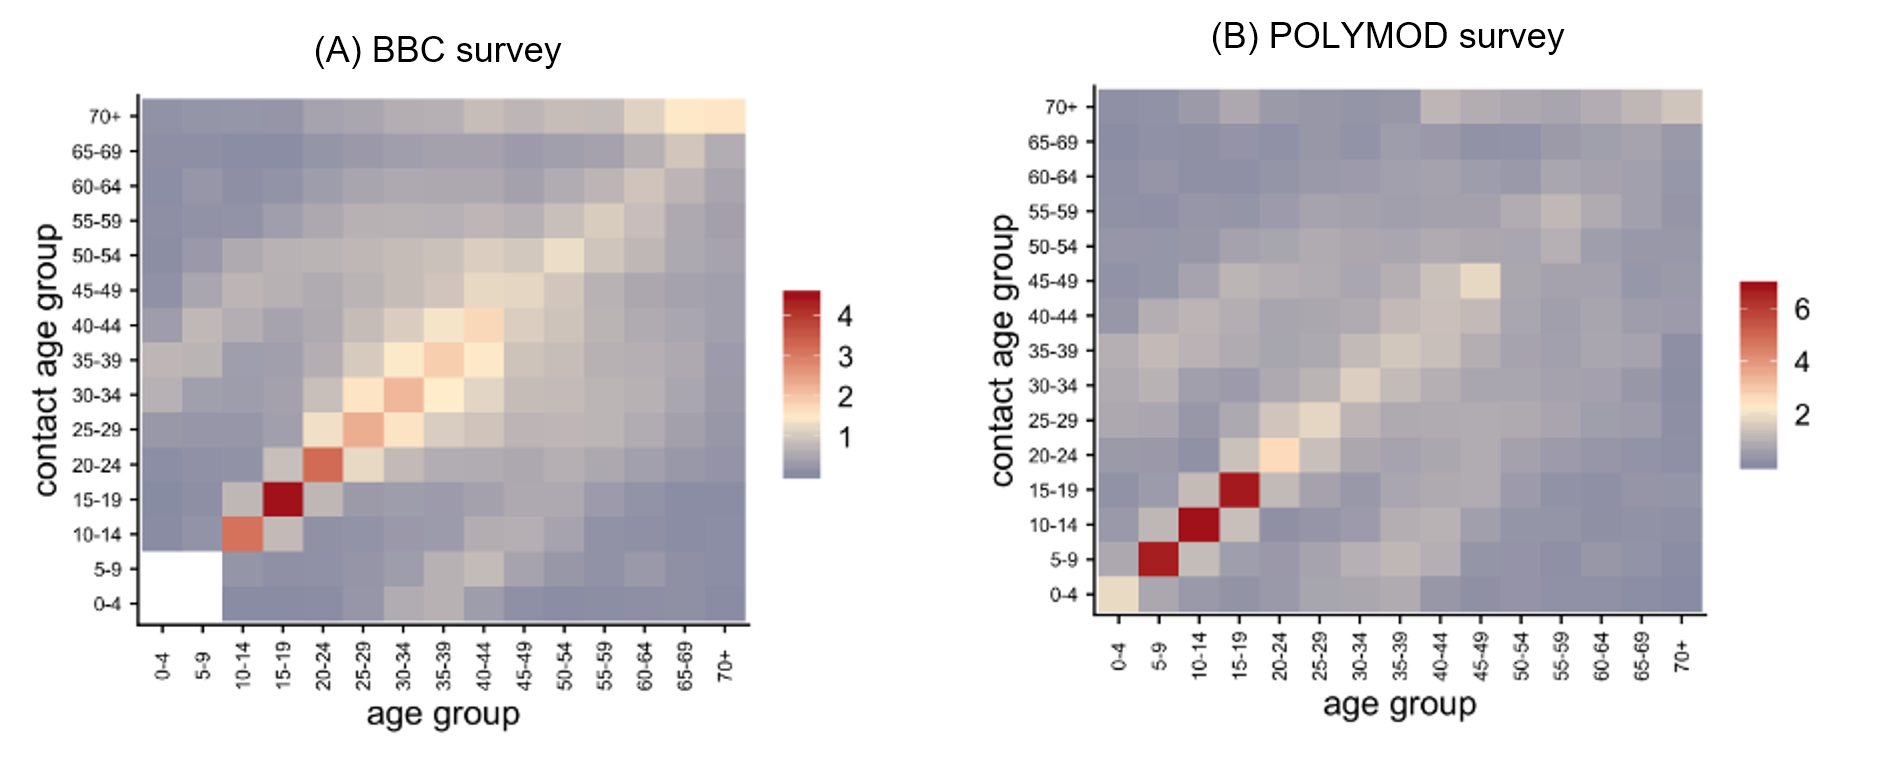
\includegraphics[width=0.9\paperwidth]{inc-prev/contact_matrices}}
  \caption[Age-based contact matrices]{Number of contacts reported between age groups in two contact surveys: (A) number of contacts reported in the POLYMOD survey~\autocite{mossongSocial}; (B) number of contacts reported in the BBC Pandemic survey~\autocite{klepacContacts}, which only collected data on those aged over 12. A clear diagonal, showing associative mixing is visible, and children have more contacts. Parallel diagonals off the main diagonal show mixing between parents and their children. Figure adapted from \textcite{klepacContacts}, licensed under \href{https://creativecommons.org/licenses/by-nc-nd/4.0/}{CC BY-NC-ND 4.0.}}
  \label{SEIR:fig:age-contacts}
\end{figure}

\section{Prevalence process} \label{inc-prev:sec:prevalence-process}

The relationship between incidence and prevalence can be derived by considering the probability that an individual is prevalent at any time following an infection.
%I define the period the individual is prevalent for as their \emph{infection episode}.
%I index infection episodes with $i$.
%Denote the time that the infection episode begins as $B_i$ and the time it ends as $E_i \geq B_i$.
%The individual is prevalent during the interval $[B_i, E_i]$ (\ie including $B_i$ and $E_i$).
%The duration of the infection episode, the number of days for which they are prevalent, is $D_i = E_i - B_i + 1$.
%I assume that the $D_i$s are iid, with a discrete distribution defined by $\prob(D_i = d) = f_D(d)$ for $d = 1, \dots, d_\text{max}$, for some maximum episode length $d_\text{max}$, and $\prob(D_i = d) = 0$ otherwise.
%Denote by $F_D$ the cdf of $D_i$, that is $F_D(d) = \prob(D_i \leq d)$.
From this, we can derive the relationship between incidence and prevalence.

Denote by $R_{t,t'}$ the number of infection episodes with $B_i=t$ and $E_i=t'$.
For any infection beginning at $t$, the probability that it ends at $t'$ is $\prob(E_i = t' \mid B_i = t) = \prob(D_i = t' - t + 1 \mid B_i = t) = f_D(t' - t + 1)$.
Since I assume these durations are independent, the number of episodes of each duration is multinomially distributed~\autocite{paganoHIV}.
Specifically:
\begin{align}
\begin{bmatrix}
  R_{t,t} \\ R_{t,t+1} \\ \vdots \\ R_{t,t+d_\text{max}-1}
\end{bmatrix} \mid Z_t
\sim \MN \left(
  Z_t, 
  \begin{bmatrix}
    f_D(1) \\ f_D(2) \\ \vdots \\ f_D(d_\text{max})
  \end{bmatrix}
\right).
\end{align}
Now, denote by $P_{t_z,t_p}$ the number of individuals infected at $t_z$ and prevalent at $t_p$.
Formally, $P_{t_z,t_p}$ is the infection episodes with $B_i = t_z$ and $E_i \geq t_p$.
$P_{t_z,t_p}$ is $Z_{t_z}$ minus those that recover before $t_p$ (\ie at or up to $t_p - 1$).
Hence:
\begin{align}
    P_{t_z,t_p} = \begin{cases}
      0 &t_p < t_z\\
      Z_{t_z} - \sum_{i=0}^{t_p-t_z-1} R_{t_z,t_z+i} &t_z \leq t_p < t_z + d_\text{max}\\
      0 &t_p \geq t_z + d_\text{max}.
  \end{cases} \label{inc-prev:eq:Ptt-to-R}
\end{align}
Finally, express $P_t$ as the total number of people prevalent at time $t$, regardless of when they were infected.
The zeroes in \cref{inc-prev:eq:Ptt-to-R} determine the sum's limits.
\begin{align}
  P_t
  &= \sum_{t_z=-\infty}^\infty P_{t_z,t} \\
  &= \sum_{i=0}^{\dmax-1} P_{t-i,t} \label{inc-prev:eq:Pt-to-Ptt} \\
  &= \sum_{i=0}^{\dmax-1} \left(Z_{t_z} - \sum_{j=0}^{i-1} R_{t-i,t-i+j} \right) &\text{by \cref{inc-prev:eq:Ptt-to-R}}\label{inc-prev:eq:Pt-to-Rtt}.
\end{align}

In general, all the random variables in this section are dependent.
This is because they are linked by the $Z_t$s, which are themselves dependent (as explained in \cref{inc-prev:sec:infection-process}).
However, if we condition on the vector of incidence, $\vec{Z} = (Z_1, Z_2, \dots)^T$, then we will induce some independence.
This reduces the stochasticity to only that attributable to the prevalence process.
In particular, because the duration of infection episodes is independent, $R_{t_z,t_p}$ and $R_{t_z',t_p'}$ will be independent if $t_z \neq t_z'$; importantly, this holds even if $t_p = t_p'$.
Therefore, $P_{t_z,t_p}$ and $P_{t_z',t_p'}$ will be independent if $t_z \neq t_z'$.

In \cref{inc-prev:sec:observation-process} I will show that only $\E(P_t \mid \vec{Z})$ and bounds on $\V(P_t \mid \vec{Z})$ will be relevant for inferring incidence.
I know derive these from their constituent parts.

Start by considering the recoveries.
The sum of recoveries of infections that occurred on the same day $t$ is the sum of multinomial cell probabilities, and hence binomially distributed~\autocite{alamAnalysis}.
Specifically:
\begin{align}
  \sum_{i=0}^{t'} R_{t,t+i} \mid \vec{Z} &\sim \text{Binomial}(Z_t, F_D(t'+1)). \label{inc-prev:eq:binomialRt}
\end{align}
Therefore:
\begin{align}
  \E \left( \sum_{i=0}^{t'} R_{t,t+i} \mid \vec{Z} \right) &= Z_t F_D(t'+1) \label{inc-prev:eq:EsumRt} \\
  \V \left( \sum_{i=0}^{t'} R_{t,t+i} \mid \vec{Z} \right) &= Z_t F_D(t'+1) (1 - F_D(t'+1)) \label{inc-prev:eq:VsumRt}
\end{align}
by the properties of the binomial distribution (see \cref{E-distributions}).

The first moment of $P_t$ follows.
\begin{align}
\E(P_t \mid \vec{Z})
  &= \E\left(\sum_{i=0}^{d_\text{max}-1} \left( Z_{t-i} - \sum_{j=0}^{i-1} R_{t-i,t-i+j} \right) \mid \vec{Z} \right) &\text{by \cref{inc-prev:eq:Pt-to-Rtt}}\\
  &= \sum_{i=0}^{d_\text{max}-1} \left( Z_{t-i} - \sum_{j=0}^{i-1} \E( R_{t-i,t-i+j} \mid \vec{Z}) \right) \\
  &= \sum_{i=0}^{d_\text{max}-1} \left( Z_{t-i} - Z_{t-i} F_D(i) \right) &\text{by \cref{inc-prev:eq:EsumRt}}\\
  &= \sum_{i=0}^{d_\text{max}-1} Z_{t-i} (1 - F_D(i)) \\
  &= \sum_{i=0}^{d_\text{max}-1} Z_{t-i} S(i+1) \label{inc-prev:eq:EPt}.
\end{align}

The independence structure simplifies the second moment.
\begin{align}
\V(P_t \mid \vec{Z})
  &= \V\left(\sum_{i=1}^{d_\text{max}-1} P_{t-i,t} \mid \vec{Z} \right) &\text{by \cref{inc-prev:eq:Pt-to-Ptt}} \\
  &= \sum_{i=1}^{d_\text{max}-1} \V\left(P_{t-i,t} \mid \vec{Z} \right) &\text{by the conditional independence} \\
  &= \sum_{i=1}^{d_\text{max}-1} \V\left(\sum_{j=0}^{i-1} R_{t-i,t-i+j} \mid \vec{Z} \right) &\text{by~\cref{inc-prev:eq:Ptt-to-R}}\\
  &= \sum_{i=1}^{d_\text{max}-1} Z_{t-i} F_D(i) (1 - F_D(i)) &\text{by~\cref{inc-prev:eq:VsumRt}} \\
  &\leq \sum_{i=1}^{d_\text{max}-1} Z_{t-i} (1 - F_D(i)) &\text{as $F_D \leq 1$}\\
  &= \E(P_t \mid \vec{Z}). \label{inc-prev:eq:boundVPt}
\end{align}

% The probability of being positive can be modelled in different ways depending on what assumptions are most reasonable.
% The most important assumption from a statistical perspective is the whether the probability of testing positive on a given day is independent conditional on the infection time.

% \todo[inline]{Is the discussion of this model just a distraction?}
% Assuming that the probability of testing positive depends only on the infection time implies no individual variation.
% This model is formalised as $Pr(Z_i(t) = 1 \mid B_i, Z_i(1), Z_i(2) \dots) = Pr(Z_i(t) \mid B_i) = p_{t-B_i}$, that is the probability of individual $i$ testing positive $t$ days after infection depends only on the infection start time and no other quantities.
% A slight relaxation of this model is introducing covariates, allowing some variation based on an individual's characteristics.

% The model with the most dependence between times, while remaining realistic, is a multi-state model.
% Therefore, if an individual has tested negative before the present time $t$ but after $B_i$ then they will test negative at time $t$.
% The complexity of the transitions between positive and negative can be very complex.
% I consider a slight extension to allow for the possibility of false negatives, meaning a negative test between $B_i$ and $E_i$, and that this probability may change.
% This leads to the following model.
% \begin{align}
%   \prob(Z_i(t) = 1 \mid B_i, \leq E_i) &= \begin{cases}
%     \psens(t - B_i) &B_i \leq t \leq E_i\\
%     0 &\text{otherwise}
%   \end{cases}\\
%   \prob(E_i = t \mid B_i) = f_i(B_i)
% \end{align}
% Conditional on both $B_i$ and $E_i$, then $Z_i(t)$ and $Z_i(t')$ are independent for $t \neq t'$.
% However, unlike the previous model, conditioning only on $B_i$ is not sufficient for $Z_i(t)$ and $Z_i(t')$ to be independent because each $Z_i(t)$ provides information on $E_i(t)$ (in particular, $Z_i(t) = 1$ implies $E_i > t$).
% For SARS-CoV-2, the latter model is more appropriate, although, as we shall see, the assumption that $\psens$ is independent of $t$ is violated.

The expectation in \cref{inc-prev:eq:EPt} is a discrete convolution equation in the same form as \cref{intro:eq:disease-model} with $\zeta = 1$.
% The equation is of the same form as the equation used for HIV/AIDS backcalculation, as well as being found in many other fields~\autocite[and references therein]{brookmeyerBackcalculation}.

Considering multiple values of $t$ makes \cref{inc-prev:eq:EPt} into a system of simultaneous equations.
Therefore, the system can be written in matrix form:
\begin{align}
  \E(\vec{P} \mid \vec{Z}) = \matr{S} \vec{Z}. \label{inc-prev:eq:EPt-matrix} \\
\intertext{$\matr{S}$ is a lower-triangular matrix formed from $S$:}
    (\matr{S})_{i,j} &= \begin{cases}
        S(i - j + 1) & i - \dmax - 1 \leq j \leq i \\
        0 & \text{otherwise.}
    \end{cases} \label{inc-prev:eq:Smatrix}
\end{align}
In \cref{E-backcalc}, I will need to solve for this system for $\vec{Z}$ given a known $\hat{P} = \E(\vec{P} \mid {Z})$.
As $\matr{S}$ is lower-triangular, I use forward-substitution~\autocite{cormenMatrix}.
Forward-substitution sequentially solves the $t$th element of $\vec{Z}$ ($t = 1, \dots, T$) by calculating:
\begin{align}
Z_t
&= \frac{\hat{P}_t - \sum_{i=1}^{t-1} S_{ti} Z_i}{S_{tt}} \\
&= \hat{P}_t - \sum_{i=1}^{t-1} S(t - i + 1) Z_i.
\label{inc-prev:eq:forward-substitute}
\end{align}

% Numerical methods for solving systems of this form, that is solving for $\vec{Z}$ (non-random in this expression) for a known $\E (\vec{P} \mid \vec{Z} )$, are well-established~\autocite[e.g.][section 8.2]{highamAccuracy}.
% However, these algorithms can be unstable, meaning that numerical errors are large.
% This is a particular issue if $S(1)$ is small.
% Since, by definition, $S(1)=1$ here, this is not an issue in this context.
%However, if instead of estimating the incidence of RT-PCR positives, the aim was to estimate the incidence of infections, then $S(1)$ would be small and this would be an issue.
%While this quantity is more epidemiologically relevant, the time from infection to RT-PCR positivity is short and, for now, I will neglect the difference.

Unlike an inference procedure which infers the parameters simultaneously, there is no feedback loop: the value of $Z_{t}$ does not affect $Z_{t'}$ for $t' < t$.
The second term here is the contribution of the incidence prior to day $t$ to day $t$'s prevalence.
The remainder of the prevalence on day $t$ is therefore due to incidence on day $t$.
% Forward substitution is numerically stable unless the diagonal elements, here $S(1)$, are small relative to the off-diagonal elements, here $S(i)$ for $i > 0$~\autocite[section 8.2]{highamAccuracy}.
% Here, the diagonal is $S(1) = 1$ and hence the matrix the solution is numerically stable.

The variance in \cref{inc-prev:eq:boundVPt} is upper bounded by \cref{inc-prev:eq:EPt}, a fact that will prove useful in \cref{inc-prev:sec:observation-process}.
\Cref{inc-prev:eq:EPt} shows that knowledge of the survival function, $S$, is crucial to modelling the prevalence process.

\section{Observation process} \label{inc-prev:sec:observation-process}

% A \emph{prevalence survey} is a survey that tests a sample of the population for the presence of an infection.
% Series of prevalence surveys are the form of measuring prevalence that this thesis is concerned with.
% This thesis aims to infer the incidence rate from prevalence surveys.
% I use Bayesian inference, therefore the data contributes through the likelihood.
The previous sections have explained the processes leading to the population prevalence.
However, we do not directly observe the population prevalence but a sample of it.
The sampling is described mathematically by the observation process.
The survey design considered here reflects the CIS, although it would be applicable to many prevalence surveys.

On day $t$ (for $t = 1, \dots, T$), a prevalence survey such as the CIS samples $n_t$ individuals at random from the population of interest and tests if they are prevalent.
Therefore, I model the number of positive tests, $X_t$, as $X_t \mid P_t, n_t, \Npop \dist \Bin(n_t, P_t/\Npop)$.
The conditioning on $n_t$ and $\Npop$ is implicit in what follows.
These quantities are fixed by the study design and population choice, and hence I assume independent of independent of $P_t$ and $Z_t$.

The $X_t$s are conditionally independent, given the population prevalences at each time, $\vec{P} = (P_1, \dots, P_t)^T$. 
%For now, I assume that the sample is chosen uniformly at random from the population of interest.
%Assume that the surveys are independent of each other and $\vec{Z}$, conditional on the population prevalence at that time.
%The population prevalence is a latent quantity.
I will use prevalence surveys to infer incidence.
I base this inference on the likelihood, $p(\vec{x} \mid \vec{Z})$.% = \int p(\vec{x} \mid \vec{P}) p(\vec{P} \mid \vec{Z}) d\vec{P} = \int \prod_t p(x_t \mid P_t) p(\vec{P} \mid \vec{Z}) d\vec{P}$, where $\vec{x} = (x_1, x_2, \dots)^T$.
Here $\vec{x} = (x_1, \dots, x_T)$ is the vector of observed number of positive tests in the prevalence survey on each day and $\vec{Z} = (Z_{-\dmax}, Z_{-\dmax+1} \dots, Z_T)$ is the vector of incidence on each day.
The incidence back to day $-\dmax$ will affect $P_1$ and therefore need to be included in $\vec{Z}$. 

This section argues that $p(\vec{x} \mid \vec{Z}) \approx \prob(\vec{X} = \vec{x} \mid \vec{P} = \E(\vec{P} \mid \vec{Z}))$.
As the $x_t$s are independent conditional on $\vec{P}$, it follows that $p(\vec{x} \mid \vec{Z}) \approx \prod_t \prob(X_t = x_t \mid P_t = \E(P_t \mid \vec{Z}))$.
This relationship will make inference for $\vec{Z}$ much simpler because the latent vector $\vec{P}$ and the dependence of the $x_t$s can be ignored.

The basis of the argument is that the first two moments of $\vec{x} \mid \vec{Z}$ and $\vec{X} \mid \vec{P} = \E(\vec{P} \mid \vec{Z})$ have negligible difference.
The first moment follows directly from the tower property of expectations.
The majority of the argument is to show that the variance-covariance matrix $\V(\vec{X} \mid \vec{Z}) \approx \V(\vec{X} \mid \vec{P} = \E(P \mid Z))$.
There are two steps to this argument.
I start with the diagonal elements, the variances.
I show that $\V(X_t \mid \vec{Z}) \approx \V(X_t \mid \vec{P} = \E(\vec{P} = \vec{Z}))$.
The conditional independence of the $x_t$s implies that the conditional covariances are 0.
Therefore, I show that the correlation between $X_t$ and $X_{t'}$ conditional only on $\vec{Z}$ is negligible.

Starting with the variances, by the law of total variance:
\begin{align}
  &\var\left( X_t \mid \vec{Z} \right) \\
    &= \var\left[\E\left( X_t \mid \vec{Z}, \vec{P} \right) \mid \vec{Z} \right] + \E\left[\var\left( X_t \mid \vec{Z}, \vec{P} \right) \mid \vec{Z} \right] \\
    &= \var\left( n_t \frac{P_t}{\Npop} \mid \vec{Z} \right) + \E\left( n_t \frac{P_t}{\Npop} \left(1 - \frac{P_t}{\Npop} \right) \mid \vec{Z} \right) \\
    &= \left( \frac{n_t}{\Npop} \right)^2 \var\left(P_t \mid \vec{Z} \right) + \frac{n_t}{\Npop} \E\left(P_t \mid \vec{Z} \right)  - \frac{n_t}{\Npop^2} \E\left(P_t^2 \mid \vec{Z} \right) \\
    &= \left( \frac{n_t}{\Npop} \right)^2 \var\left(P_t \mid \vec{Z} \right) + \frac{n_t}{\Npop} \E\left(P_t \mid \vec{Z} \right)  - \frac{n_t}{\Npop^2} \left(\E\left(P_t \mid \vec{Z} \right) ^ 2 + \V(P_t \mid \vec{X})\right) \\
    &= \frac{n_t(n_t - 1)}{\Npop^2} \var\left(P_t \mid \vec{Z} \right) + n_t \frac{\E\left(P_t \mid \vec{Z} \right)}{\Npop}\left(1 - \frac{\E\left(P_t \mid \vec{Z} \right)}{\Npop} \right) \\
    &= \frac{n_t(n_t - 1)}{\Npop^2} \var\left(P_t \mid \vec{Z} \right) + \V(X_t \mid P_t = \E(P_t \mid \vec{Z})).
\end{align}
The first term of this expression is negligible in the contexts I consider.
These contexts have $n_t << \Npop$.
$\Npop$ is the population of England (around 56 million) while $n_t$ is the daily sample size (10s of thousands).
Further $\V(P_t \mid \vec{Z}) \leq \E(P_t \mid \vec{Z})$ (\cref{inc-prev:eq:boundVPt}).
Therefore, $\var\left( X_t \mid \vec{Z} \right) \approx \V(X_t \mid P_t = \E(P_t \mid \vec{Z}))$.

A similar argument will show that the correlation between $x_t$ and $x_{t'}$ ($t \neq t'$) is negligible.
The basic structure of this argument is as the previous one.
The result follows because the observation noise dominates, and this is uncorrelated.
In the following, all are implicitly conditioned on $\vec{Z}$.
However, for clarity I omit the conditioning from the notation.
\begin{align}
  &\lvert \cor(X_t, X_{t'}) \rvert \\
  &= \frac{\lvert\cov(X_t, X_{t'})\rvert}{\sqrt{\var(X_t) \var(X_{t'})}} &\text{by definition}\\
  &= \frac{\lvert \E(\cov(X_t, X_{t'} \mid \vec{P})) + \cov(\E(X_t \mid \vec{P}), \E(X_{t'} \mid \vec{P})) \rvert}{\sqrt{\var(X_t) \var(X_{t'})}} &\text{by law of total covariance} \\
  &= \frac{\lvert 0 + \cov(n_t P_t / \Npop, n_{t'} P_{t'} / \Npop) \rvert}{\sqrt{\var(X_t) \var(X_{t'})}} \\
  &= \frac{n_t n_{t'} \lvert \cov(P_t, P_{t'}) \rvert}{\Npop^2 \sqrt{\var(X_t) \var(X_{t'})}}  \\
  &<< \frac{n_t n_{t'} \lvert \cov(P_t, P_{t'}) \rvert}{\Npop^2 \sqrt{\var(P_t) \var(P_{t'})}} &\text{as $\V(X_t) >> \V(P_t)$} \\
  &= \frac{n_t n_{t'}}{\Npop^2} \lvert \cor(P_t, P_{t'}) \rvert &\text{by def of $\cor$}\\
  &\leq \frac{n_t n_{t'}}{\Npop^2} &\text{as $\lvert \cor(\cdot) \rvert \leq 1$}.
\end{align}
$n_t n_{t'} / \Npop^2$ is very small, for the same reason that $n_t / \Npop$ is small.
The argument above shows that $\lvert \cor(X_t, X_{t'}) \rvert$ is much smaller than this.
Therefore, neglecting the correlation between $X_t$ and $X_{t'}$ is a good approximation.

This section showed that, when using a prevalence survey such as CIS, the likelihood $p(\vec{x} \mid \vec{z})$ is very well approximated by $p(\vec{x} \mid \vec{P} = \E(\vec{P} \mid \vec{z}))$.


\section{Conclusion} \label{inc-prev:sec:conclusion}

Robust, unbiased prevalence estimates already exist (\cref{E-intro:sec:cis}), and incidence estimates are the objective of this thesis.
This chapter has shown that the key quantity relating these quantities is the distribution of the duration of RT-PCR positivity.
However, no estimates of this quantity in the general population exist (see \cref{E-intro:sec:previous-duration-estimates}).
Therefore, I now turn to estimating the duration of RT-PCR positivity.

\ifSubfilesClassLoaded{
  \listoftodos
}{}

\end{document}